\documentclass[12pt]{article} 
\usepackage{minted}
\usepackage[utf8]{inputenc}
\usepackage[T1]{fontenc}
\usepackage[english]{babel}
\usepackage{amsmath}
\usepackage{amsfonts}
\usepackage{url}
\usepackage{fancyhdr}
\pagestyle{fancy}
\usepackage{appendix}
\usepackage{graphicx}
\usepackage{caption}
\usepackage{geometry}
\usepackage{csquotes}
\usepackage{algorithm}
\usepackage{algpseudocode}
\usepackage[table]{xcolor}
\usepackage{xcolor}
\usepackage{listings}
\lstset{basicstyle=\ttfamily,
  showstringspaces=false,
  commentstyle=\color{red},
  keywordstyle=\color{blue}
}

\geometry{hmargin=2.5cm, vmargin=2.5cm}

\DeclareMathOperator*{\argmin}{arg\,min}

\setlength{\headheight}{15pt}
\addtolength{\topmargin}{-3pt}

\pagestyle{fancy}
\fancyhf{}
\fancyheadoffset{0pt}
\fancyfootoffset{0pt}
\fancyhead[L]{\leftmark}
\fancyhead[R]{}
\fancyfoot[C]{\thepage}
\begin{document}
\begin{titlepage}
  \noindent
  
\includegraphics[width=0.35\textwidth]{assets/logo-ligne-simple-couleur-master.png}\hfill
  
\includegraphics[width=0.35\textwidth]{assets/univ.jpg}

  \vfill

\begin{center}
  {\fontfamily{qpl} \Large {Rapport de Projet}}
\end{center}

  \noindent\rule{\textwidth}{0.6pt}
  \begin{center}
    {\LARGE \textbf{WeatherScope}}\par
  \end{center}
  \noindent\rule{\textwidth}{0.6pt}

\begin{center}
  {\large Big Data and NoSQL}
\end{center}

  \vspace{1.2cm}

  \noindent
  \makebox[0.5\textwidth][l]{\large Réalisé par}%
  \makebox[0.5\textwidth][r]{\large Encadré par}\par
  \vspace{0.2cm}
  \noindent
  \makebox[0.5\textwidth][l]{\large DITER Justin \& SANCHEZ Louise}%
  \makebox[0.5\textwidth][r]{\large Mme. AKID-ZEKRI Hajer}

  \vfill

  \begin{center}
    {\large \textit{Master 2 Informatique Parcours Systèmes Logiciels et Calculs Distribués}}\par
    \vspace{0.2cm}
    {\large \textit{Université Côte d'Azur - Année 2026-2027}}
  \end{center}
\end{titlepage}

\newpage
\thispagestyle{empty}
\section*{\centering \small Résumé}
\hspace*{0.75cm} Ce rapport présente ....
\newpage
\thispagestyle{empty}
\section*{\centering \small Abstract}
\hspace*{0.75cm} This report studies .....



\newpage
\thispagestyle{empty}
\tableofcontents
\newpage

\section{Introduction}
Ce projet s'inscrit dans le cadre ....
\section{Périmètre Géographique, Temporalité \& Provenance des Données}
\label{sec:perimetre}

\subsection{Périmètre d'étude}

\paragraph{Données.}
Toutes les observations viennent de GHCN-Daily, l'archive quotidienne de la NOAA~\cite{menne2012}. Les métadonnées ont été récupérées le 8 novembre 2026~; l'URL, la date et le SHA-256 de chaque fichier sont dans \texttt{data/raw/metadata/MANIFEST.json}. La sélection se refait avec \texttt{scripts/select\_stations.py}.

\paragraph{Zones.}
Le Michigan regroupe les stations américaines avec le code d'État \texttt{MI}. Le sud de l'Allemagne regroupe les stations situées en Bavière ou en Bade-Wurtemberg, d'après les frontières de Natural Earth~\cite{naturalearth}. Les deux zones ont une surface proche (environ 146\,000 et 106\,000~km\textsuperscript{2}). Nous écartons les stations allemandes au-dessus de 800~m (18 stations, dans les Alpes et la Forêt-Noire), car la neige y dépend surtout de l'altitude~; le Michigan ne dépasse pas 523~m. Les latitudes ne sont pas identiques~: la moitié des stations du Michigan sont au sud de 43,0°N, la moitié des allemandes au nord de 48,8°N (figure~\ref{fig:carte}).

\paragraph{Période.}
Nous étudions 1991--2020, la normale climatique actuelle de l'OMM~\cite{wmo2017}. La référence pour les anomalies (F3) est 1961--1990~; elle passe par le même chargement mais est comptée à part. Un hiver va de décembre à février~: 30 hivers, de 1990--91 à 2019--20.

\paragraph{Stations.}
Nous gardons les stations qui ont des données TMAX, TMIN ou PRCP sur 1991--2020 (tableau~\ref{tab:stations}). Les réseaux diffèrent~: au Michigan, 675 stations viennent de CoCoRaHS, un réseau de bénévoles~\cite{cifelli2005}, et la plupart n'existent que depuis 2005. En Allemagne, le réseau (ECA\&D~\cite{kleintank2002}) reste stable. Une moyenne sur toutes les stations montrerait donc surtout l'arrivée de nouvelles stations. Pour les tendances, nous n'utilisons que les 269 stations \guillemotleft~à longue série~\guillemotright{}, qui couvrent toute la période. Elles suffisent pour les minimums du sujet~: plus de 100 stations, et au plus 2,9 millions de couples station--jour pour 200\,000 demandés. L'inventaire ne donne que la première et la dernière année~: les trous seront vérifiés après chargement.

La hauteur de neige (SNWD) est disponible dans les deux zones. Les chutes de neige (SNOW) n'existent qu'au Michigan.

\begin{table}[h!]
  \centering
  \small
  \begin{tabular}{lrr}
    \hline
     & Michigan & Sud de l'Allemagne \\
    \hline
    Stations de la zone & 1\,560 & 400 \\
    Stations retenues & 1\,058 & 295 \\
    \quad dont à longue série & 119 & 150 \\
    \quad dont débutées en 2005 ou après & 763 & 18 \\
    \hline
    \multicolumn{3}{l}{\emph{Stations retenues par élément~: avec données / sur toute la période}} \\
    TMAX & 317 / 95 & 264 / 93 \\
    TMIN & 319 / 98 & 264 / 94 \\
    PRCP & 1\,045 / 117 & 294 / 148 \\
    SNOW & 1\,009 / 109 & -- \\
    SNWD & 890 / 110 & 287 / 140 \\
    \hline
  \end{tabular}
  \caption{Stations retenues sur 1991--2020 (inventaire NOAA du 8/11/2026).}
  \label{tab:stations}
\end{table}

\begin{figure}[h!]
  \centering
  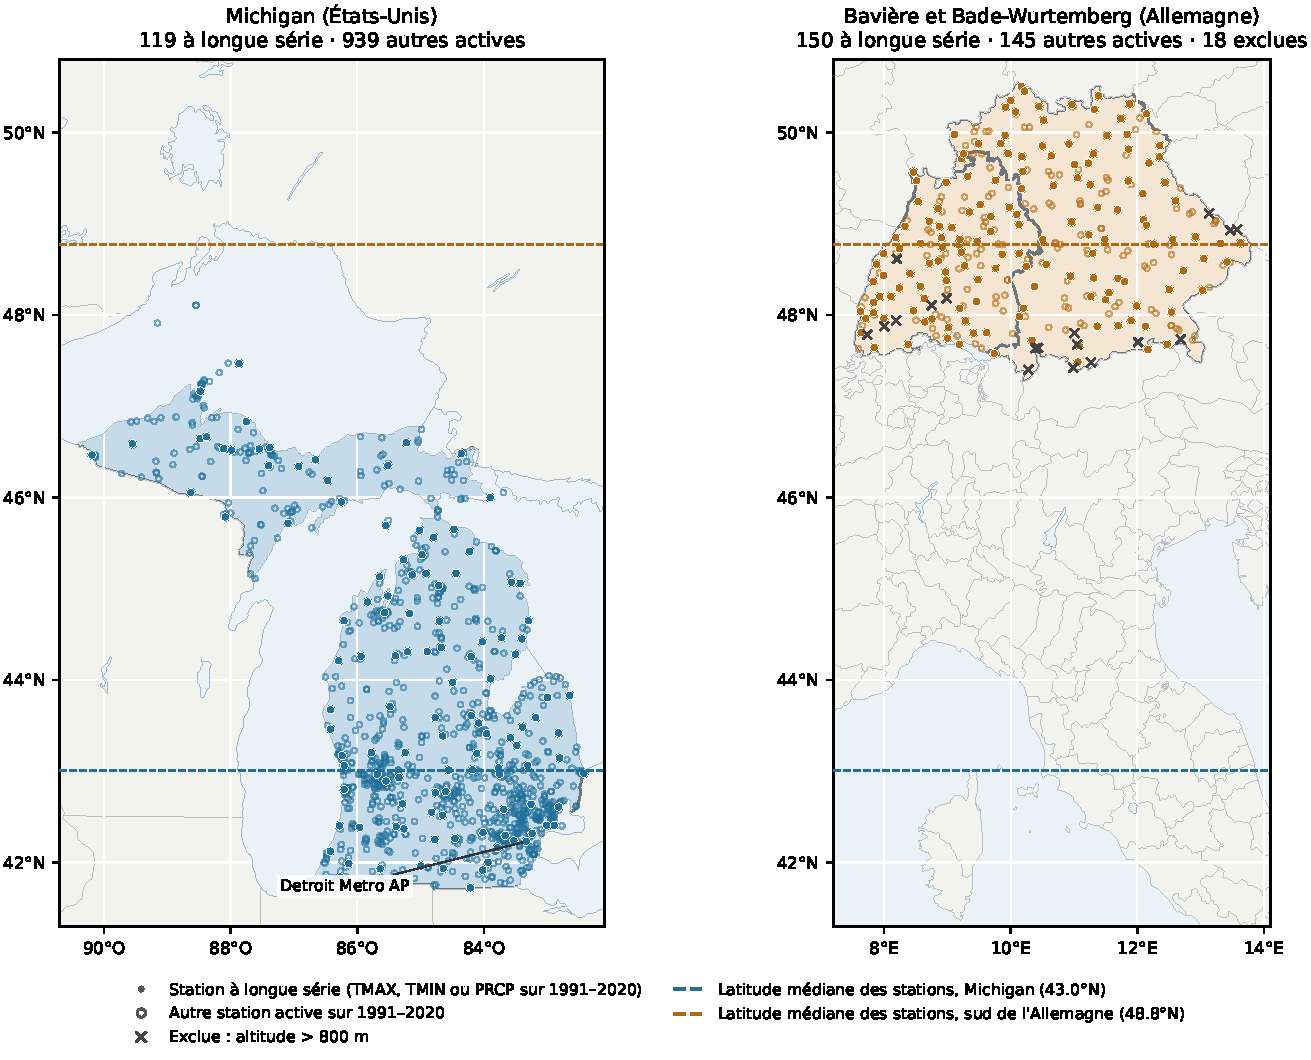
\includegraphics[width=0.8\textwidth]{assets/carte_zones.pdf}
  \caption{Stations retenues, à la même échelle. Pointillés~: latitude médiane des stations de chaque zone.}
  \label{fig:carte}
\end{figure}

% TODO 2.2~: heure d'observation (7 h ou 17 h au Michigan) et conséquences pour les comparaisons.

\subsection{Traçabilité, Traitement des Drapeaux (Flags) et Valeurs Manquantes}

\section{Architecture Système \& Implémentation des Services}


\section{Conclusion}

Dans ce Projet ...



\newpage
\thispagestyle{empty}
%\listoffigures

\newpage
\thispagestyle{empty}
\begin{thebibliography}{9}

\end{thebibliography}

\appendix

\end{document}